\documentclass[journal,12pt,twocolumn]{IEEEtran}
%
\usepackage{setspace}
\usepackage{multicol}
\usepackage{gensymb}
\usepackage{enumerate}
\usepackage{xcolor}
\usepackage{caption}
%\usepackage{subcaption}
%\doublespacing
\singlespacing
%\usepackage{epstopdf}
%\usepackage{graphicx}
%\usepackage{amssymb}
%\usepackage{relsize}
\usepackage[cmex10]{amsmath}
\usepackage{mathtools}
%\usepackage{amsthm}
%\interdisplaylinepenalty=2500
%\savesymbol{iint}
%\usepackage{txfonts}
%\restoresymbol{TXF}{iint}
%\usepackage{wasysym}
\usepackage{amsthm}
\usepackage{mathrsfs}
\usepackage{txfonts}
\usepackage{stfloats}
\usepackage{cite}
\usepackage{cases}
\usepackage{subfig}
%\usepackage{xtab}
\usepackage{longtable}
\usepackage{multirow}
%\usepackage{algorithm}
%\usepackage{algpseudocode}
%\usepackage{enumitem}
\usepackage{mathtools}
\usepackage{iithtlc}
%\usepackage[framemethod=tikz]{mdframed}
\usepackage{listings}
\usepackage{amsmath}
\usepackage{polynomial}
\usepackage{url}
\def\UrlBreaks{\do\/\do-}
%\usepackage{stmaryrd}


%\usepackage{wasysym}
%\newcounter{MYtempeqncnt}
\DeclareMathOperator*{\Res}{Res}
%\renewcommand{\baselinestretch}{2}
\renewcommand\thesection{\arabic{section}}
\renewcommand\thesubsection{\thesection.\arabic{subsection}}
\renewcommand\thesubsubsection{\thesubsection.\arabic{subsubsection}}

\renewcommand\thesectiondis{\arabic{section}}
\renewcommand\thesubsectiondis{\thesectiondis.\arabic{subsection}}
\renewcommand\thesubsubsectiondis{\thesubsectiondis.\arabic{subsubsection}}

% correct bad hyphenation here
\hyphenation{op-tical net-works semi-conduc-tor}

\lstset{
language=Python,
frame=single, 
breaklines=true
}

%\lstset{
	%%basicstyle=\small\ttfamily\bfseries,
	%%numberstyle=\small\ttfamily,
	%language=python,
	%backgroundcolor=\color{white},
	%%frame=single,
	%%keywordstyle=\bfseries,
	%%breaklines=true,
	%%showstringspaces=false,
	%%xleftmargin=-10mm,
	%%aboveskip=-1mm,
	%%belowskip=0mm
%}

%\surroundwithmdframed[width=\columnwidth]{lstlisting}


\begin{document}
%

\theoremstyle{definition}
\newtheorem{theorem}{Theorem}[section]
%\newtheorem{problem}{Problem}[section]
\newtheorem{problem}{Problem}
\newtheorem{proposition}{Proposition}
%\newtheorem{proposition}{Proposition}[section]
\newtheorem{lemma}{Lemma}[section]
\newtheorem{corollary}[theorem]{Corollary}
\newtheorem{example}{Example}[section]
%\newtheorem{definition}{Definition}[section]
\newtheorem{definition}{Definition}
%\newtheorem{definition}{Definition}
%\newtheorem{algorithm}{Algorithm}[section]
%\newtheorem{cor}{Corollary}
\newcommand{\BEQA}{\begin{eqnarray}}
\newcommand{\EEQA}{\end{eqnarray}}
\newcommand{\define}{\stackrel{\triangle}{=}}

\bibliographystyle{IEEEtran}
%\bibliographystyle{ieeetr}

\providecommand{\nCr}[2]{\,^{#1}C_{#2}} % nCr
\providecommand{\nPr}[2]{\,^{#1}P_{#2}} % nPr
\providecommand{\mbf}{\mathbf}
\providecommand{\pr}[1]{\ensuremath{\Pr\left(#1\right)}}
\providecommand{\qfunc}[1]{\ensuremath{Q\left(#1\right)}}
\providecommand{\sbrak}[1]{\ensuremath{{}\left[#1\right]}}
\providecommand{\lsbrak}[1]{\ensuremath{{}\left[#1\right.}}
\providecommand{\rsbrak}[1]{\ensuremath{{}\left.#1\right]}}
\providecommand{\brak}[1]{\ensuremath{\left(#1\right)}}
\providecommand{\lbrak}[1]{\ensuremath{\left(#1\right.}}
\providecommand{\rbrak}[1]{\ensuremath{\left.#1\right)}}
\providecommand{\cbrak}[1]{\ensuremath{\left\{#1\right\}}}
\providecommand{\lcbrak}[1]{\ensuremath{\left\{#1\right.}}
\providecommand{\rcbrak}[1]{\ensuremath{\left.#1\right\}}}
\theoremstyle{remark}
\newtheorem{rem}{Remark}
\newcommand{\sgn}{\mathop{\mathrm{sgn}}}
\providecommand{\abs}[1]{\left\vert#1\right\vert}
\providecommand{\res}[1]{\Res\displaylimits_{#1}} 
\providecommand{\norm}[1]{\lVert#1\rVert}
\providecommand{\mtx}[1]{\mathbf{#1}}
\providecommand{\mean}[1]{E\left[ #1 \right]}
\providecommand{\fourier}{\overset{\mathcal{F}}{ \rightleftharpoons}}
%\providecommand{\hilbert}{\overset{\mathcal{H}}{ \rightleftharpoons}}
\providecommand{\system}{\overset{\mathcal{H}}{ \longleftrightarrow}}
	%\newcommand{\solution}[2]{\textbf{Solution:}{#1}}
\newcommand{\solution}{\noindent \textbf{Solution: }}
\providecommand{\dec}[2]{\ensuremath{\overset{#1}{\underset{#2}{\gtrless}}}}
%\numberwithin{equation}{section}
\numberwithin{equation}{problem}

%\numberwithin{problem}{subsection}
%\numberwithin{definition}{subsection}
\makeatletter
\@addtoreset{figure}{problem}
\makeatother

\let\StandardTheFigure\thefigure
%\renewcommand{\thefigure}{\theproblem.\arabic{figure}}
\renewcommand{\thefigure}{\theproblem}


%\numberwithin{figure}{subsection}

\def\putbox#1#2#3{\makebox[0in][l]{\makebox[#1][l]{}\raisebox{\baselineskip}[0in][0in]{\raisebox{#2}[0in][0in]{#3}}}}
     \def\rightbox#1{\makebox[0in][r]{#1}}
     \def\centbox#1{\makebox[0in]{#1}}
     \def\topbox#1{\raisebox{-\baselineskip}[0in][0in]{#1}}
     \def\midbox#1{\raisebox{-0.5\baselineskip}[0in][0in]{#1}}

\vspace{3cm}

\title{ 
\logo{
Numerical Solution of Ordinary Differential Equations
}
}

\author{G V V Sharma$^{*}$ %<-this  stops a space
\thanks{*The author is with the Department
of Electrical Engineering, IIT, Hyderabad
502285 India e-mail: gadepall@iith.ac.in. All material in the manuscript is released under GNU GPL.  Free to use for all.}% <-this % stops a space
}



% make the title area
\maketitle

%\newpage

%\tableofcontents


\IEEEpeerreviewmaketitle

\bigskip

\begin{abstract}
Through examples, this manual discusses the numerical solution of ordinary differential equations (ODE)
by Taylor
series method,  Euler's Method, Euler's modified method and Runge-Kutta
Methods.  Python codes are provided for all these methods.
\end{abstract}
%
\section{Taylor Series Method}
\begin{definition}
\label{def:taylor}
The Taylor series of $f(x)$ that is infinitely differentiable at $a$ is the power series
\begin{multline}
\label{eq:taylor}
f(x) = f(a) + \frac{f^{1}(a)}{1!} \brak{x-a}+  \frac{f^{2}(a)}{2!}\brak{x-a}^2
\\
+ \frac{f^{3}(a)}{3!}\brak{x-a}^3+\dots
\end{multline}
where $f^{n}(a)$ is the $n$th derivative of $f$ at $a$.
%
\end{definition}
%\section{Limit}
\begin{problem}
Find the 2nd and 3rd derivative of $y$ using the following differential equation.
\begin{equation}
\label{eq:ode}
y^{(1)} = 1 - xy, \quad y(0) = 1
\end{equation}
where 
$y^{(1)} = \frac{dy}{dx}$.
\end{problem}
\solution From \eqref{eq:ode}, through successive differentiation,
\begin{align}
\label{eq:taylor_der}
y^{(2)} &= -xy^{(1)} - y 
\\
y^{(3)} &=  -xy^{(2)} -2y^{(1)} 
\label{eq:taylor_mod_der}
\end{align}
%
\begin{problem}
Express \eqref{eq:ode}
as a difference equation using the Taylor series method.  Assume a step size $h$.
\end{problem}
%
\solution
Substituting $x = a+h$ in \eqref{eq:taylor} \cite{taylor},
%
\begin{multline}
\label{eq:taylor_mod}
f(a+h) = f(a) + \frac{f^{1}(a)}{1!} h+  \frac{f^{2}(a)}{2!}h^2
\\
+ \frac{f^{3}(a)}{3!}h^3+\dots
\end{multline}
%
From \eqref{eq:taylor},
Let $f(a) = y_n, f(a+h) = y_{n+1}$.  From \eqref{eq:ode} - \eqref{eq:taylor_mod}, the desired difference equation is
\begin{equation}
\label{eq:taylor_diff}
y_{n+1} = y_n + \frac{y_n^{(1)}}{1!} h+  \frac{y_n^{(2)}}{2!}h^2
+ \frac{y_n^{(3)}}{3!}h^3+\dots
\end{equation}
where 
\begin{align}
x_0 &= 0, 
y_0 = 1
\\
x_{n+1} &= x_{n}+h
\\
y_n^{(1)} &= 1-x_ny_n
\\
y_n^{(2)} &= -x_ny_n^{(1)} - y_n 
\\
y_n^{(3)} &=  - x_ny_n^{(2)} -2y_n^{(1)} 
\end{align}
\begin{problem}
Compute and plot $y$ for $x \in \brak{0,5}$ with 25 subintervals using \eqref{eq:taylor_diff}.
\end{problem}
\solution The following script plots the output in Fig. \ref{fig:taylor}
\lstinputlisting{./codes/taylor.py}
\begin{figure}[!h]
\centering
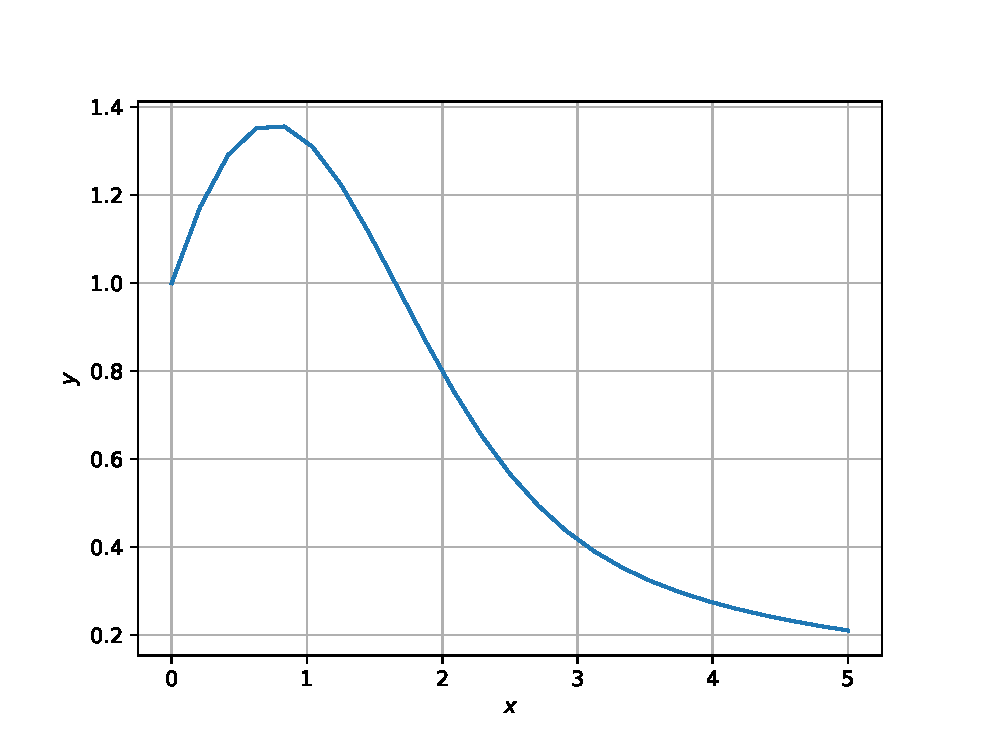
\includegraphics[width=\columnwidth]{./figs/taylor.eps}
\caption{Taylor series method.}
\label{fig:taylor}
\end{figure}
%
\section{Euler's Method}
\begin{problem}
Formulate a difference equation for \eqref{eq:ode} using the Euler method.
\end{problem}
\solution \eqref{eq:ode} can be expressed as \cite{euler}
%
\begin{align}
\label{eq:euler_diff}
\frac{y_{n+1}-y_n}{h} &\approx 1 - x_ny_n, 
\\
\implies y_{n+1} &= y_n + h\brak{1 - x_ny_n}, \quad y_0 = 1
\end{align}
%
using the definition of the derivative.
\begin{problem}
Compute and plot $y$ using \eqref{eq:euler_diff}.
\end{problem}
\solution
 The following script plots the output in Fig. \ref{fig:euler}
\lstinputlisting{./codes/euler.py}
\begin{figure}[!h]
\centering
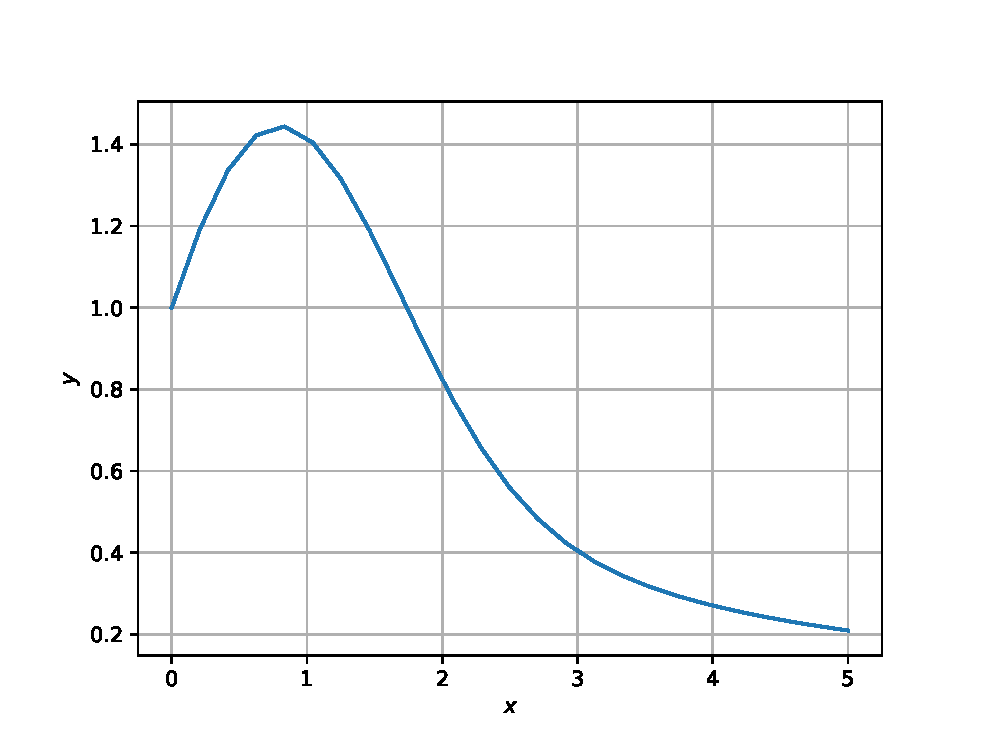
\includegraphics[width=\columnwidth]{./figs/euler.eps}
\caption{Euler's method}
\label{fig:euler}
\end{figure}
\section{Euler's Modified Method}
\begin{problem}
Show that the differential equation
\begin{align}
\label{eq:ode_def}
y^{(1)}(t) = f\brak{t,y(t)}
\end{align}
results in the approximation
\begin{equation}
\label{eq:euler_modfied}
y(t+h) \approx y(t) + h f\brak{t + \frac{h}{2}, y(t)+ \frac{h}{2}f(t,y(t))}
\end{equation}
%can be approximated as
%\begin{equation}
%y^{(1)}(t) \approx f\brak{t + \frac{h}{2},y(t) + \frac{h}{2}f\brak{t,y(t)}}
%\end{equation}
for small values of $h$.
\end{problem}
\begin{proof}
Using the definition of the deritave,
%
\begin{align}
\label{eq:taylor_one}
y\brak{t + h} &\approx y(t) + hy^{(1)}\brak{t}
\\
y^{(1)}\brak{t+\frac{h}{2}} &\approx  y(t) + \frac{h}{2}y^{(1)}\brak{t}
\\
&=y(t) + \frac{h}{2}f\brak{t + \frac{h}{2}, y(t)+ \frac{h}{2}f(t,y(t))}
\label{eq:taylor_two}
\end{align}
using \eqref{eq:ode_def}.
From Fig. \ref{fig:midpoint} \cite{midpoint}, 
\begin{align}
y^{(1)}(t) &\approx y^{(1)}\brak{t+\frac{h}{2}}
\end{align}
resulting in \eqref{eq:euler_modfied} by substituting \eqref{eq:taylor_two} in \eqref{eq:taylor_one}.
\end{proof}
%
\begin{figure}[!h]
\centering
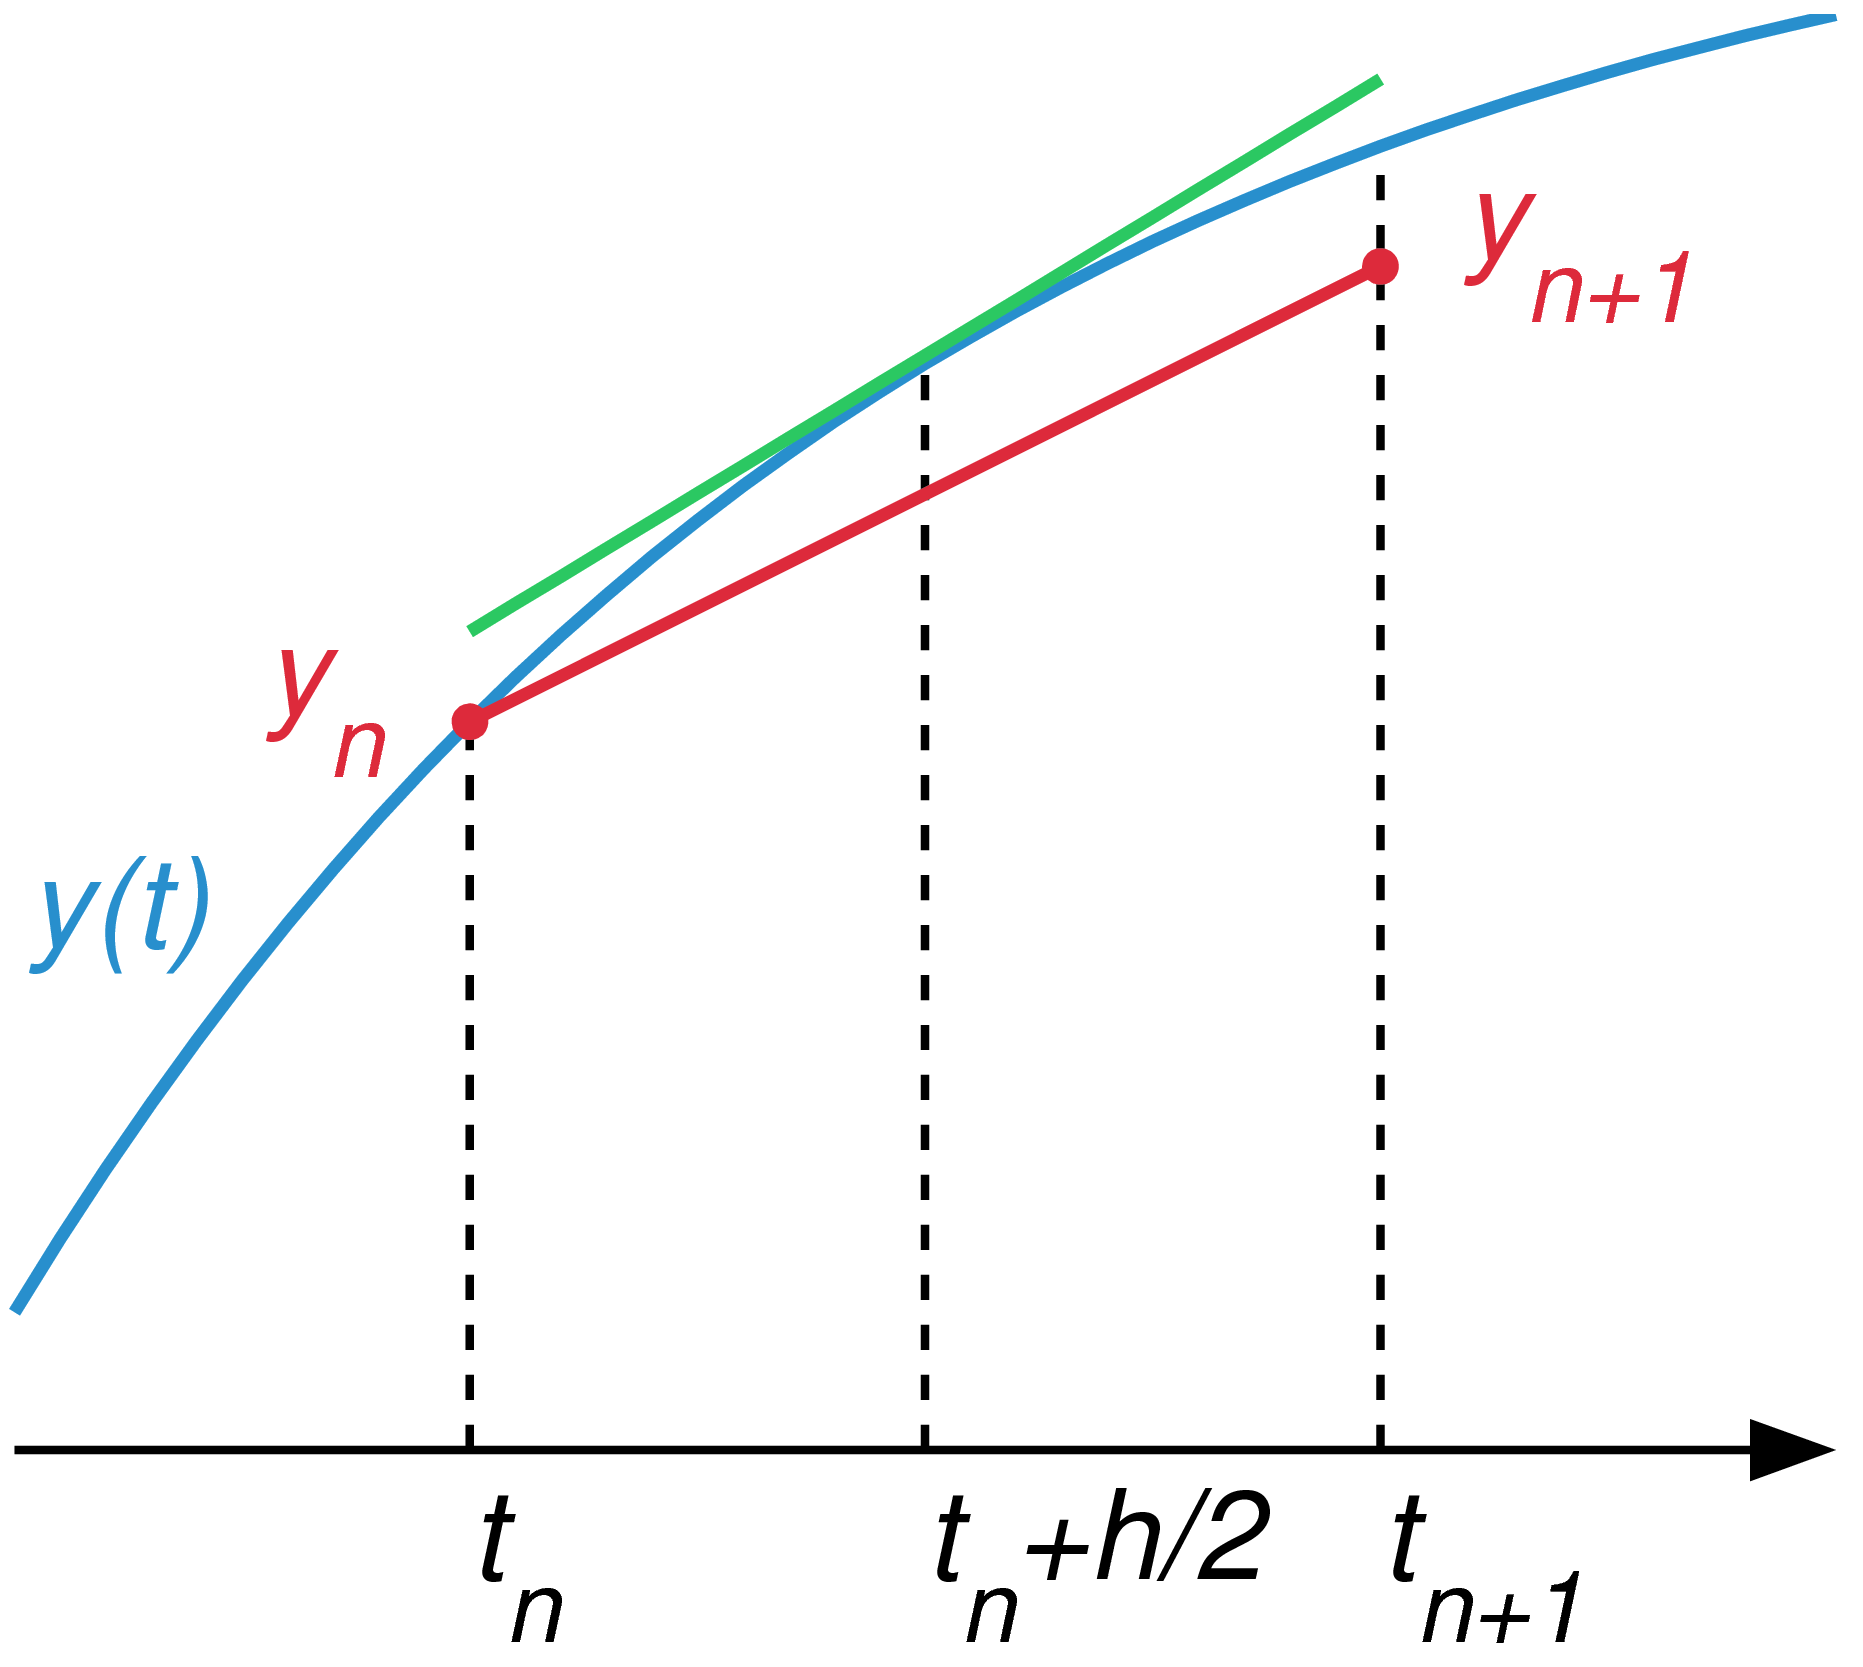
\includegraphics[width=\columnwidth]{./figs/midpoint.eps}
\caption{}
\label{fig:midpoint}
\end{figure}
%
\begin{problem}
Formulate a difference equation for the modified Euler method.
\end{problem}
\solution From \eqref{eq:euler_modfied} \cite{midpoint},
\begin{align}
\label{eq:euler_modified_diff}
y_{n+1} &= y_n + h f\brak{x_n + \frac{h}{2}, y_n+ \frac{h}{2}f(x_n,y_n)}
\\
x_{n+1} &= x_n + h
\end{align}
\begin{problem}
Compute and plot $y$ using \eqref{eq:euler_modified_diff}.
\end{problem}
\solution
 The following script plots the output in Fig. \ref{fig:euler_modified}
\lstinputlisting{./codes/euler_modified.py}
\begin{figure}[!h]
\centering
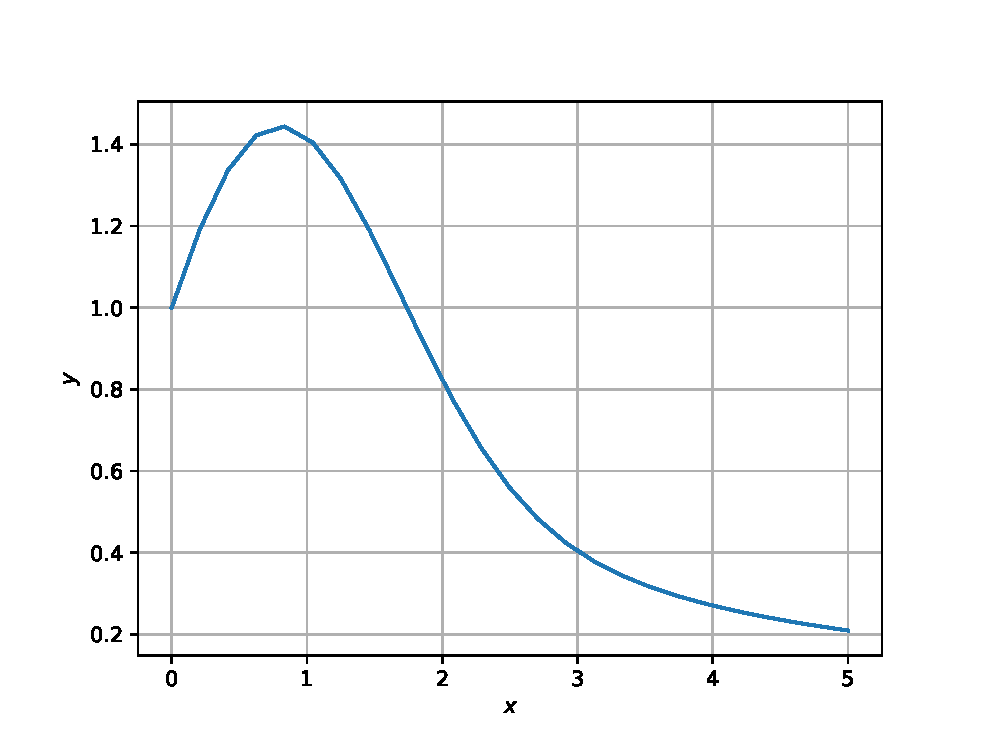
\includegraphics[width=\columnwidth]{./figs/euler_modified.eps}
\caption{Euler's modified method.}
\label{fig:euler_modified}
\end{figure}
%
\section{The Runge-Kutta method}
\begin{problem}
Obtain the difference equation for \eqref{eq:ode_def} using the Runge-Kutta method. 
\end{problem}
\solution The desired equation is given by \cite{runge}
%
\begin{align}
\label{eq:runge_diff}
y_{n+1} &= y_{n}+{\tfrac {h}{6}}\left(k_{1}+2k_{2}+2k_{3}+k_{4}\right),
\\
x_{n+1} &= x_{n}+h,
\end{align}
%
where
\begin{align}
k_{1}&=f(x_{n},y_{n}),\\k_{2}&=f\left(x_{n}+{\frac {h}{2}},y_{n}+h{\frac {k_{1}}{2}}\right),\\k_{3}&=f\left(x_{n}+{\frac {h}{2}},y_{n}+h{\frac {k_{2}}{2}}\right),\\k_{4}&=f\left(x_{n}+h,y_{n}+hk_{3}\right).
\end{align}
%
\begin{problem}
Compute and plot $y$ using \eqref{eq:runge_diff}.
\end{problem}
\solution
 The following script plots the output in Fig. \ref{fig:runge}
\lstinputlisting{./codes/runge.py}
\begin{figure}[!h]
\centering
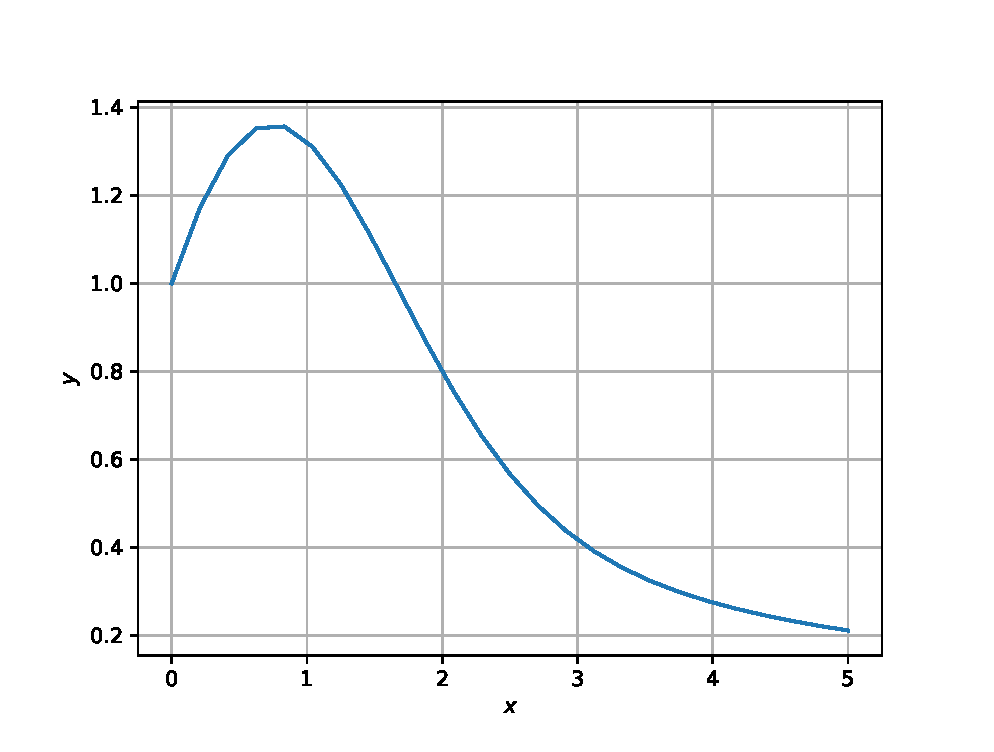
\includegraphics[width=\columnwidth]{./figs/runge.eps}
\caption{Runge-Kutta method.}
\label{fig:runge}
\end{figure}
%
\bibliography{IEEEabrv,gvv_num_ode}
\end{document}


